% Chapter Template

\chapter{Signal Region Optimisation} % Main chapter title

\label{Chapter5} % Change X to a consecutive number; for referencing this chapter elsewhere, use \ref{ChapterX}

\lhead{Chapter 5. \emph{Signal Region Optimisation}} % Change X to a consecutive number; this is for the header on each page - perhaps a shortened title

%----------------------------------------------------------------------------------------
%	SECTION 1
%----------------------------------------------------------------------------------------
\section{Hadronic pre selection}
In order to maximise sensitivity to a wide range of signal models the final analysis bins must be carefully chosen. Previously, \scalht regions and jet categories where used to categorise events. For Run 2 a different approach is being considered. In this section when the \scalht bin for each particular cjet and btag category is considered this will be denoted as \scalhtcat.


\section{Strategy in Run 1}

In the previous analysis selected events are categorised using the jet and btag multiplicities and split into \scalht regions (hadronic pre selection). The QCD multijet background will be several orders of magnitude larger than the expected signal. Using an \alphat requirement of $\alphat > 0.55$ can reduce this to the sub percent level of the overall background. The \alphat thresholds (and the \scalht regions) used for the analysis are determined partly by the trigger thresholds. The \scalht bin dependant \alphat requirements map onto an effective lower bound on \mht. The remaining electroweak backgrounds after the \alphat requirement must then be estimated.


Considering the previous approach there are three main (related) issues that can quickly be determined. Firstly, while the \alphat variable is highly adept at removing the QCD multijet background it may not be optimal for distinguishing signal from the remaining background. Secondly, each bin can have only one \alphat (and therefore \mht) threshold and no advantage may be taken of the shape. Thirdly, each jet category has the same \alphat threshold per \scalht bin. Higher jet multiplicities lead to lower \alphat values and so more flexibility should significantly improve the situation.


\section{Improvements for Run 2}

In order to address the issues raised above a new strategy has been adopted. Firstly using an improved trigger strategy the \alphat thresholds per bin have been reduced to keep the minimum \mht requirement around $130 GeV$ (shown in \ref{tab:alphat-thresholds}). \footnote{From a QCD contamination study undertaken using data from Run 1 this is the lowest threshold for effective QCD suppression \cite{ANYTHING}. QCD contamination will be extensively studied when data from Run 2 is available}. This maximises the possible acceptance using the \alphat variable. To then optimise sensitivity for each \scalhtcat bin several variables which make use of missing energy were investigated. As there are $30 (categories) \times7 (ht regions) = 210 bins$ choosing these thresholds manually is not feasible. An automated binning procedure which accounts for systematic errors as well as SM yields in both the signal and control regions has been implemented for this purpose and is described below. Utilising this procedure and investigating a range of signal models allows determination of the optimal variable to use for binning.          

\begin{table}[h!]
  \caption{\alphat and (effective) \mht thresholds per \scalht bin.\label{tab:alphat-thresholds}}
  \centering
  \footnotesize
  \begin{tabular}{ lcccccc }
    \hline
    \hline
    \scalht      & 200--250   & 250--300   & 300--350  & 350--400  & 400--800 \\ %& $>$900       \\
    \hline                                                                     
    \alphat      & 0.65       & 0.60       & 0.55      & 0.53      & 0.52     \\  %& 0.505         \\
    "Min \mht"   & $\sim$128  & $\sim$138  & $\sim$125 & $\sim$133 & $\sim$137 \\  %& $\sim$126 \\
    \hline
    \hline
  \end{tabular}
\end{table}


% \begin{figure}
% \centering
%     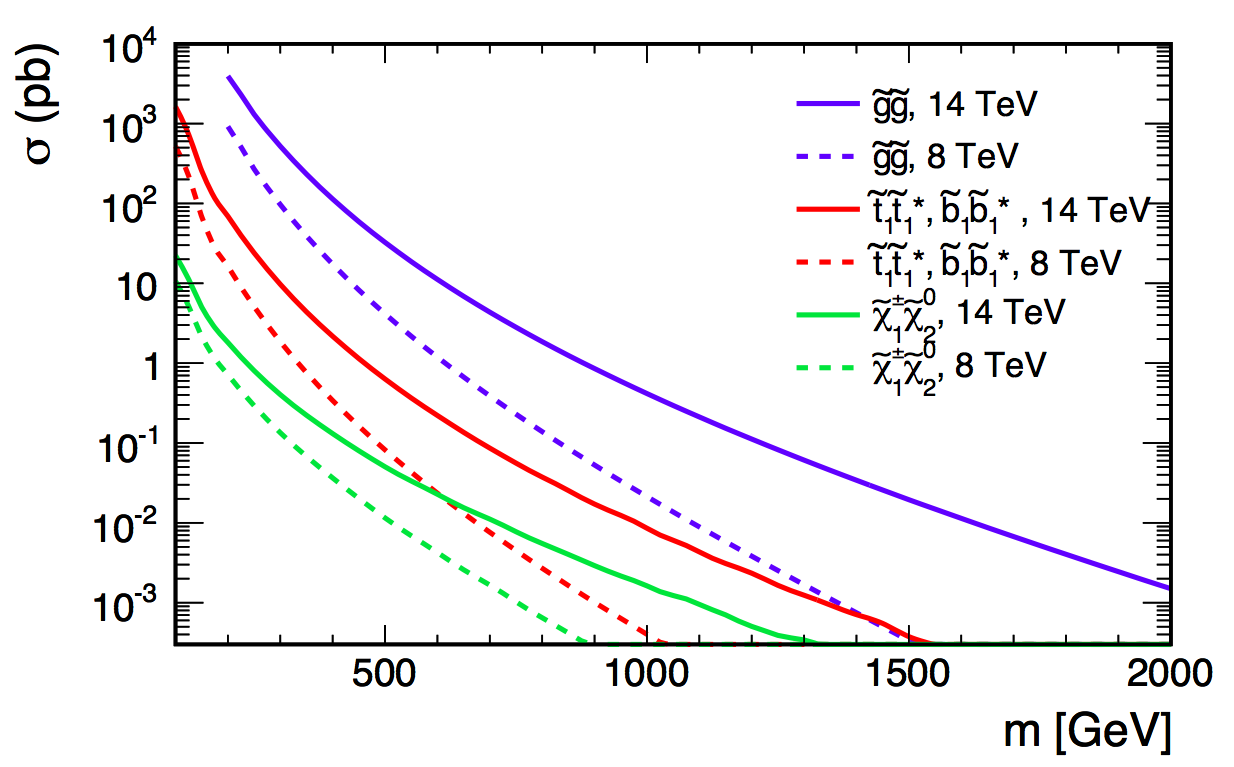
\includegraphics[width=0.7\textwidth]{Figures/snowmass.png}
%   \caption{SUSY production cross sections at 14 TeV compared with 8TeV}
%   \label{snow}
% \end{figure}


